\documentclass[a4paper,11pt]{amsart}

\usepackage{gensymb}

\usepackage{tikz}
\usetikzlibrary{arrows.meta}
\usepackage{caption}

\usepackage{times}
\usepackage[top=27mm, left=23mm, bottom=23mm, right=23mm]{geometry}
\usepackage{amsfonts, amssymb, amsgen, amsthm, amscd, amsmath}
\usepackage{mathtools}
\mathtoolsset{showonlyrefs=true}

\usepackage{bm}
%\usepackage{mathpazo}
\usepackage{domitian}
\usepackage[T1]{fontenc}
\let\oldstylenums\oldstyle

\usepackage{enumerate}
\usepackage{color}
\usepackage[all]{xy}

\newtheorem{theorem}{Theorem}[section]
\newtheorem{proposition}[theorem]{Proposition}
\newtheorem{lemma}[theorem]{Lemma}
\newtheorem{corollary}[theorem]{Corollary}
\newtheorem{claim}[theorem]{Claim}
\theoremstyle{definition}
\newtheorem{remark}[theorem]{Remark}
\newtheorem{example}[theorem]{Example}
\newtheorem{definition}[theorem]{Definition}

\newcommand{\outimes}[2]{\overset{#1}{\underset{#2}{\otimes}}}
\newcommand{\C}[1]{\mathcal{#1}}
\newcommand{\B}[1]{\mathbb{#1}}
\newcommand{\G}[1]{\mathfrak{#1}}
\newcommand{\rmod}[1]{\text{{\bf Mod}-}{#1}}

\newcommand{\Span}{\text{\rm Span}}
\newcommand{\Tor}{\text{\rm Tor}}
\newcommand{\Ind}{\text{\rm Ind}}
\newcommand{\Res}{\text{\rm Res}}
\newcommand{\Ext}{\text{\rm Ext}}
\newcommand{\Hom}{\text{\rm Hom}}
\newcommand{\CoInd}{\text{\rm CoInd}}
\newcommand{\Simp}{{\Delta}}
\newcommand{\Diff}{{\Omega}}
\newcommand{\xla}[1]{\xleftarrow{#1}}
\newcommand{\colim}{\text{colim}}
\renewcommand{\baselinestretch}{1.15}

\setlength{\parskip}{1.2mm}
\setlength{\parindent}{0mm}

\title{Electromagnetism Assignment For The Eightth Time}

\author{Haixuan Lin - 23307110267}
\email{23307110267@m.fudan.edu.cn}


\address{Fudan University, Physics Department, China}

\begin{document}
	
	\begin{abstract}
		Here is the electromagnetism assignment for the eightth time which is for the course given by professor Weitao Liu. In order to practise the expertise in scientific film of physics, students need to practise using \LaTeX to composing their own work, even if this is only a ordinary homework.
	\end{abstract}
	
	\maketitle
	\section*{Main Text}

	\subsection*{8-4}
	
	According to Kirchhoff's voltage equation
	
	$$
	\xi =Ri\left( t \right) +L\frac{\mathrm{d}}{\mathrm{d}t}i\left( t \right) +\frac{1}{C}\int_0^t{i\left( t \right) \mathrm{d}t}
	$$
	
	Take $t=0^+$ into
	
	$$
	\frac{\mathrm{d}}{\mathrm{d}t}i\left( 0^+ \right) =0
	$$
	
	In order to solve this differential equation we take Laplace Transform on it
	
	$$
	0=sRI\left( s \right) -Ri\left( 0^+ \right) +s^2LI\left( s \right) -sLi\left( 0^+ \right) -L\frac{\mathrm{d}}{\mathrm{d}t}i\left( 0^+ \right) +\frac{1}{C}I\left( s \right) 
	$$
	
	As a result
	
	$$
	\displaystyle sI\left( s \right) =i\left( 0^+ \right) \frac{s^2+\dfrac{R}{L}s}{s^2+\dfrac{R}{L}s+\dfrac{1}{LC}}
	$$
	
	Take the inverse Laplace transform
	
	$$
	\frac{\mathrm{d}}{\mathrm{d}t}i\left( t \right) =-\frac{i\left( 0^+ \right)}{LC\sqrt{\dfrac{1}{LC}-\left( \dfrac{R}{2L} \right) ^2}}e^{-\tfrac{R}{2L}t}\sin \sqrt{\frac{1}{LC}-\left( \frac{R}{2L} \right) ^2}t\qquad(t>0^+)
	$$
	
	Do a approxmation that we consider when
	
	$$
	t=\frac{1}{\sqrt{\dfrac{1}{LC}-\left( \dfrac{R}{2L} \right) ^2}}\frac{\pi}{2}
	$$
	
	We have 
	
	$$
	V_\textbf{out max}=nL\frac{i\left( 0^+ \right)}{LC\sqrt{\frac{1}{LC}-\left( \frac{R}{2L} \right) ^2}}e^{-\tfrac{R}{2L}\frac{1}{\sqrt{\frac{1}{LC}-\left( \frac{R}{2L} \right) ^2}}\tfrac{\pi}{2}}=2.1\times10^4\,\mathrm{V}
	$$
	
	\subsection*{8-7}
	
	% TODO: \usepackage{graphicx} required
	\begin{figure}
		\centering
		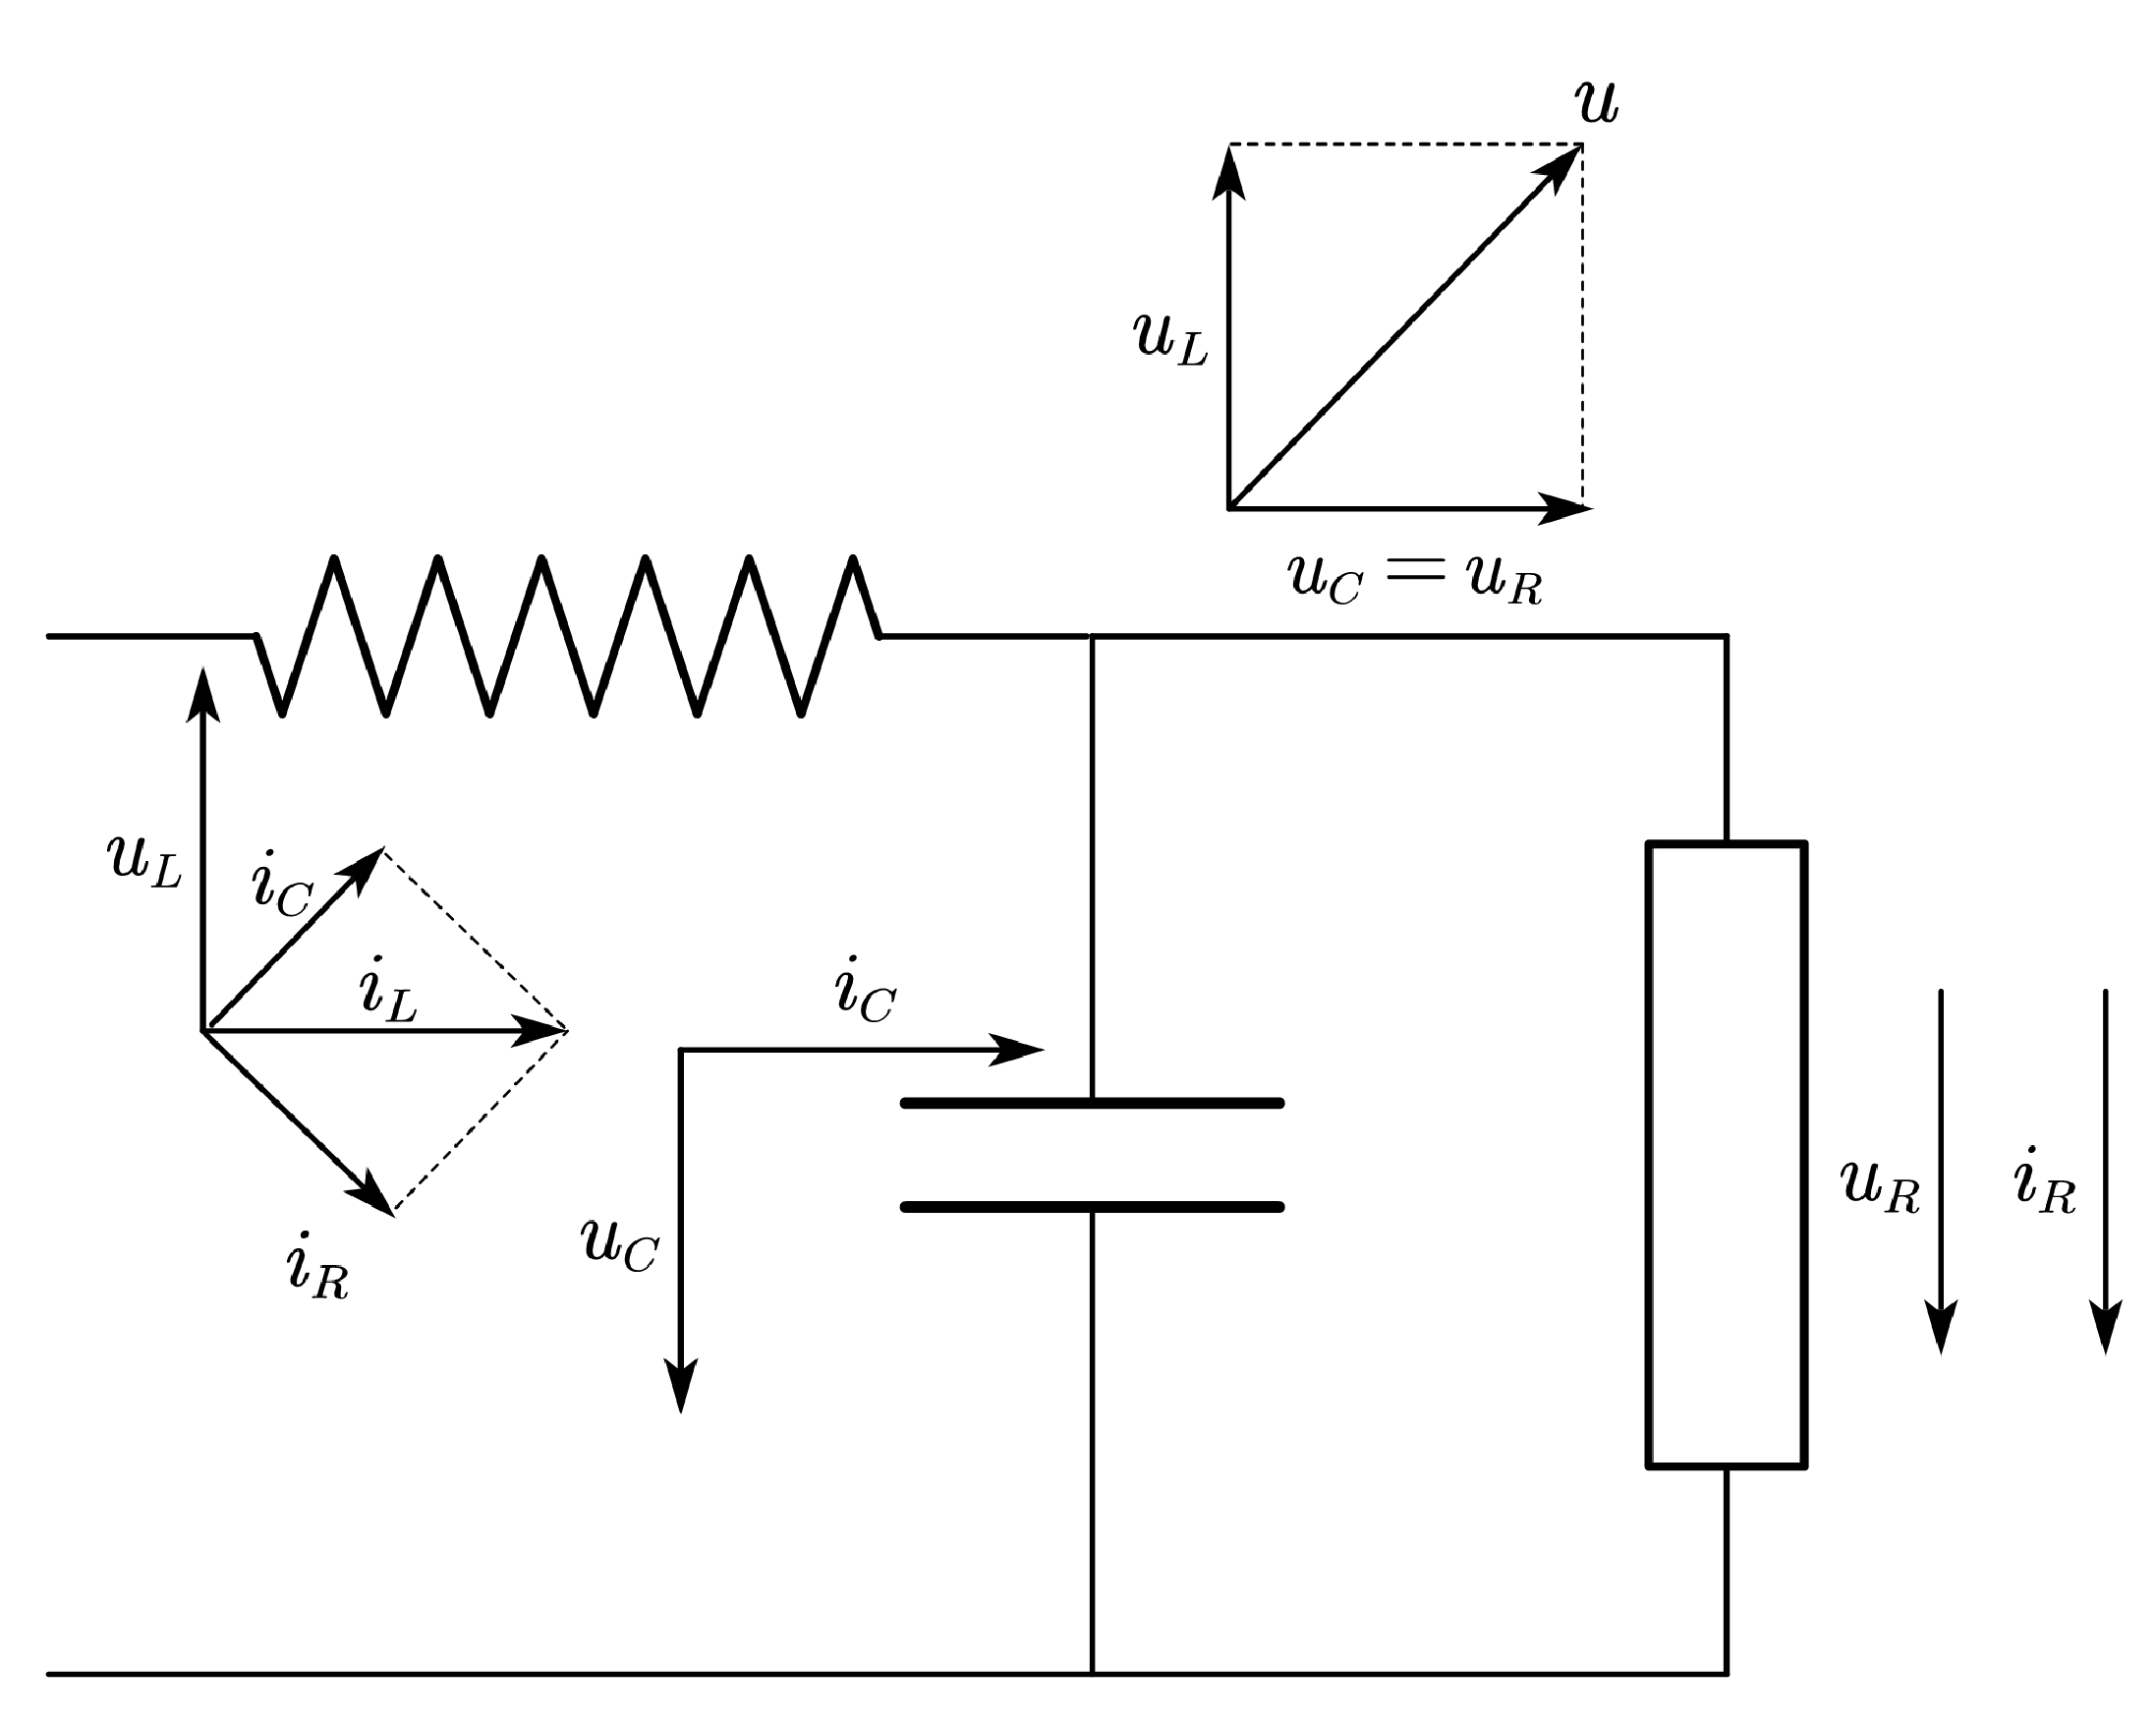
\includegraphics[width=0.7\linewidth]{8-12}
		\caption*{8-4}
		\label{fig:8-12}
	\end{figure}
	
	\subsubsection*{(1)}
	
	$$
	\angle u_C-\angle i_R=0
	$$
	
	\subsubsection*{(2)}
	
	$$
	\angle i_C-\angle i_R=\frac{\pi}{2}
	$$
	
	\subsubsection*{(3)}
	
	$$
	\angle u_R-\angle u_L=-\frac{3}{4}\pi 
	$$
	
	\subsubsection*{(4)}
	
	$$
	\angle u-\angle i=\frac{1}{4}\pi 
	$$
		
	\subsection*{8-9}
	
	According to the principle of linear superposition, the contributions of current source and voltage source are considered separately.
	
	When there is no capacitance.
	
	$$
	U_{ab\,\,\mathrm{direct}}=-E
	$$
	
	$$
	U_{ab\,\,\mathrm{alternative}}=iR_r
	$$
	
	As a result
	
	$$
	U_{ab}=-E+iR_r=-5.5\sim-6.0\,\mathrm{V}
	$$
	
	When there is capacitance.
	
	$$
	U_{ab\,\,\mathrm{direct}}=-E
	$$
	
	$$
	U_{ab\,\,\mathrm{alternative}}=\frac{i}{\sqrt{\left( 2\pi fC \right) ^2+\dfrac{1}{R_{r}^{2}}}}
	$$
	
	$$
	U_{ab}=-E+\frac{i}{\sqrt{\left( 2\pi fC \right) ^2+\dfrac{1}{R_{r}^{2}}}}=-5.85\sim -6.0\,\mathrm{V}
	$$
	
	\subsection*{8-12}
	
	We resolved the circuit using complex numbers:
	
	
	$$
	\tilde{u}_1=\frac{R}{R+R_L+\mathrm{i}\omega L}\tilde{u}
	$$
	
	$$
	\tilde{u}_2=\frac{R_1}{R_1+R_2}\tilde{u}
	$$
	
	$$
	\tilde{v}=\tilde{u}_1-\tilde{u}_2
	$$
	
	$$
	v=|\tilde{v}|=\sqrt{\left( \frac{R\left( R+R_L \right)}{\left( R+R_L \right) ^2+\omega ^2L^2}-\frac{R_1}{R_1+R_2} \right) ^2+\left( \frac{R\omega L}{\left( R+R_L \right) ^2+\omega ^2L^2} \right) ^2}u
	$$
	
	Note $\mathrm{i}=\sqrt{-1}$. In order to minimize $v$, let
	
	$$
	\frac{R\left( R+R_L \right)}{\left( R+R_L \right) ^2+\omega ^2L^2}-\frac{R_1}{R_1+R_2}=0
	$$
	
	$$
	V=v_{\min}=\frac{R\omega L}{\left( R+R_L \right) ^2+\omega ^2L^2}u_{\mathrm{effect}}
	$$
	
	As a result
	
	$$
	R_L=14\,\Omega
	$$
	
	$$
	L=89.1\,\mathrm{mH}
	$$
	
	% TODO: \usepackage{graphicx} required
	\begin{figure}[h]
		\centering
		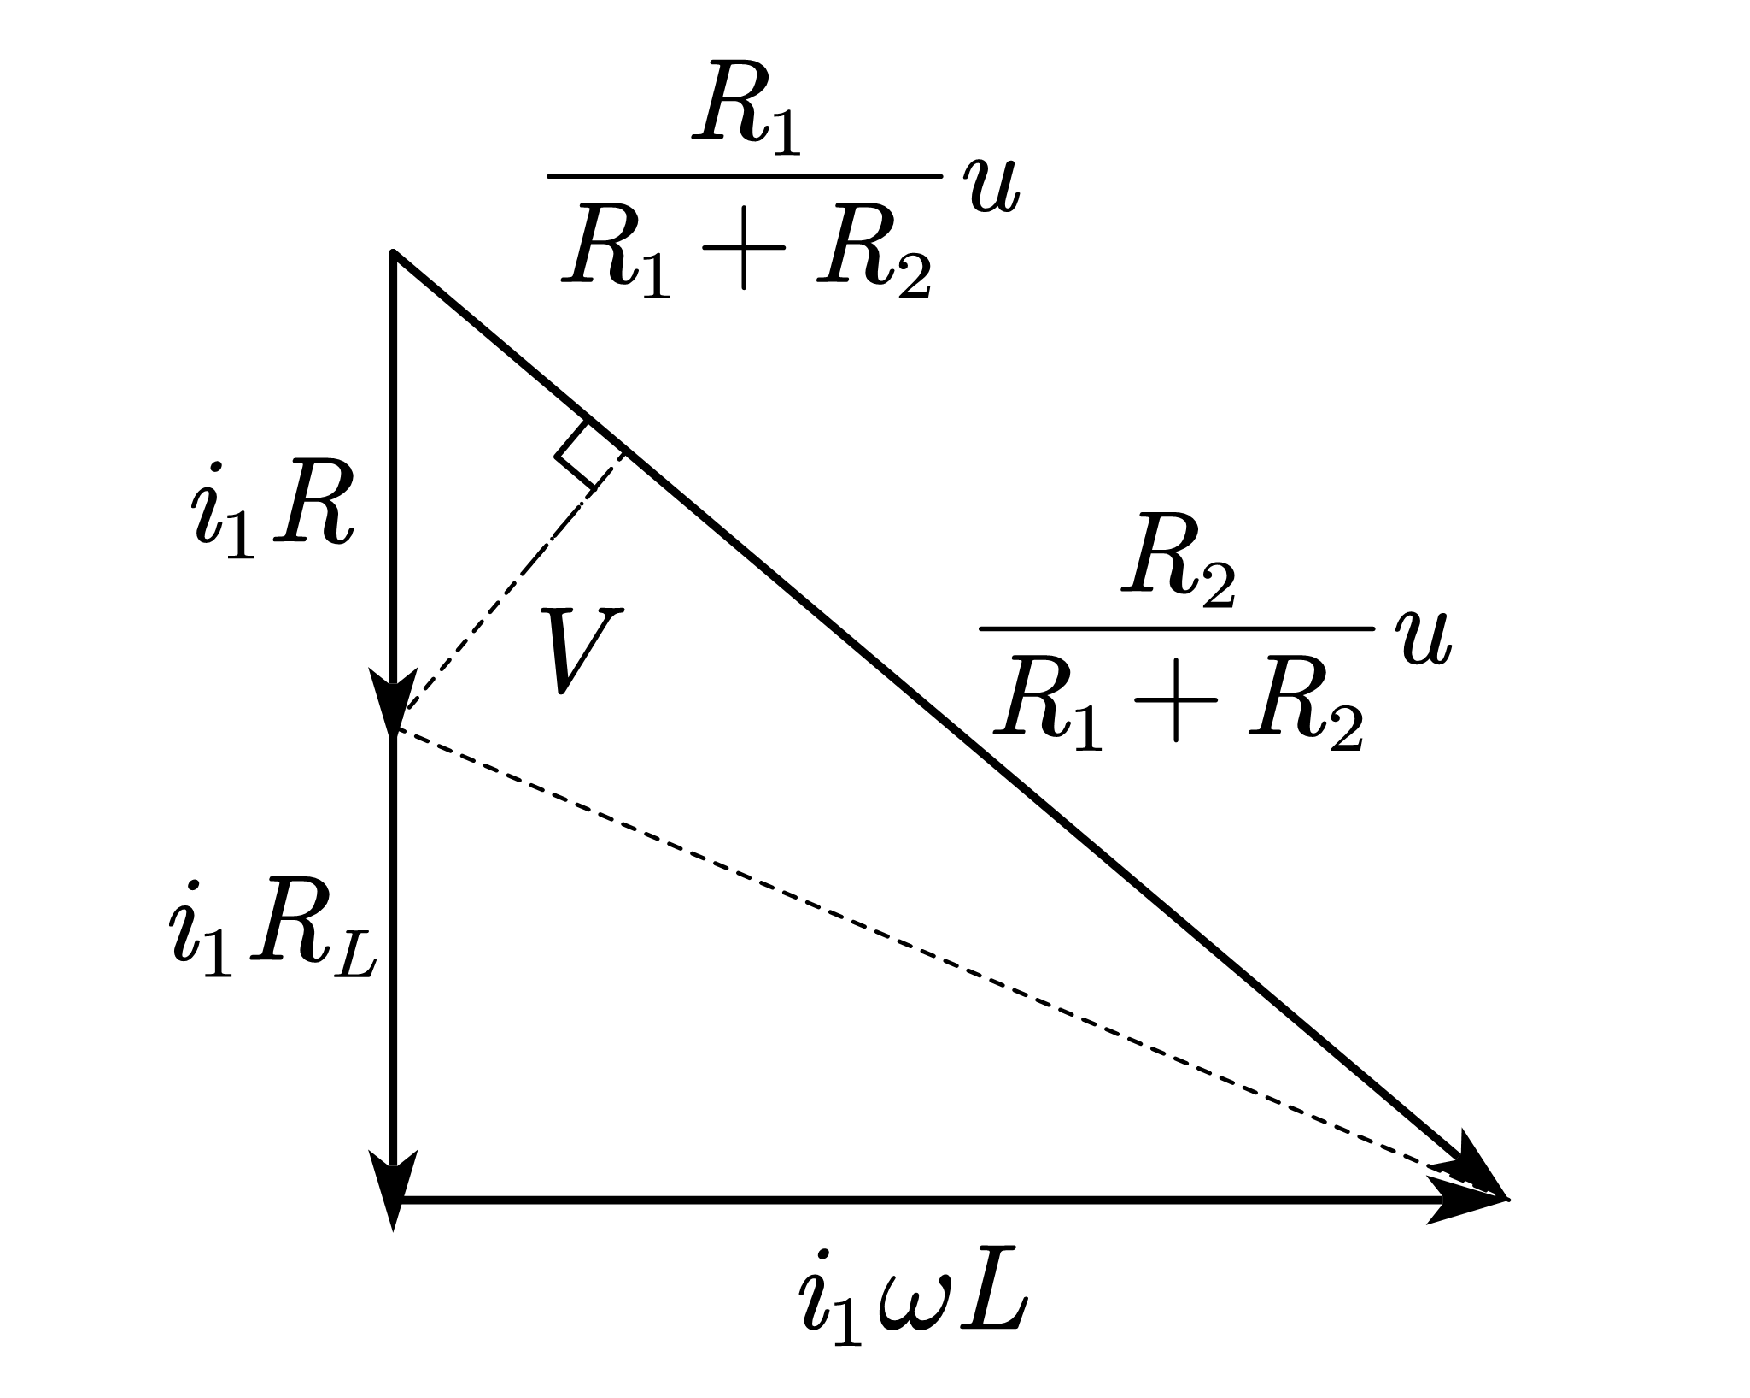
\includegraphics[width=0.7\linewidth]{8-12-12}
		\caption*{8-12}
		\label{fig:8-12-12}
	\end{figure}
	
	Or we can use graph and geometry:
	
	$$
	\left( \frac{R_1}{R_1+R_2}u \right) ^2+V^2=\left( i_1R \right) ^2
	$$
	
	$$
	\left( i_1\left( R+R_L \right) \right) ^2+\left( i_1\omega L \right) ^2=u^2
	$$
	
	$$
	\left( i_1R_L \right) ^2+\left( i_1\omega L \right) ^2=V^2+\left( \frac{R_2}{R_1+R_2}u \right) ^2
	$$
	
	We can solve this too!
	
	\subsection*{8-15}	
	
	\subsubsection*{(1)}
	
	Use defination
	
	$$
	P_W=ui\cos \varphi =24.2\,\mathrm{W}
	$$
	
	\subsubsection*{(2)}
	
	% TODO: \usepackage{graphicx} required
	\begin{figure}
		\centering
		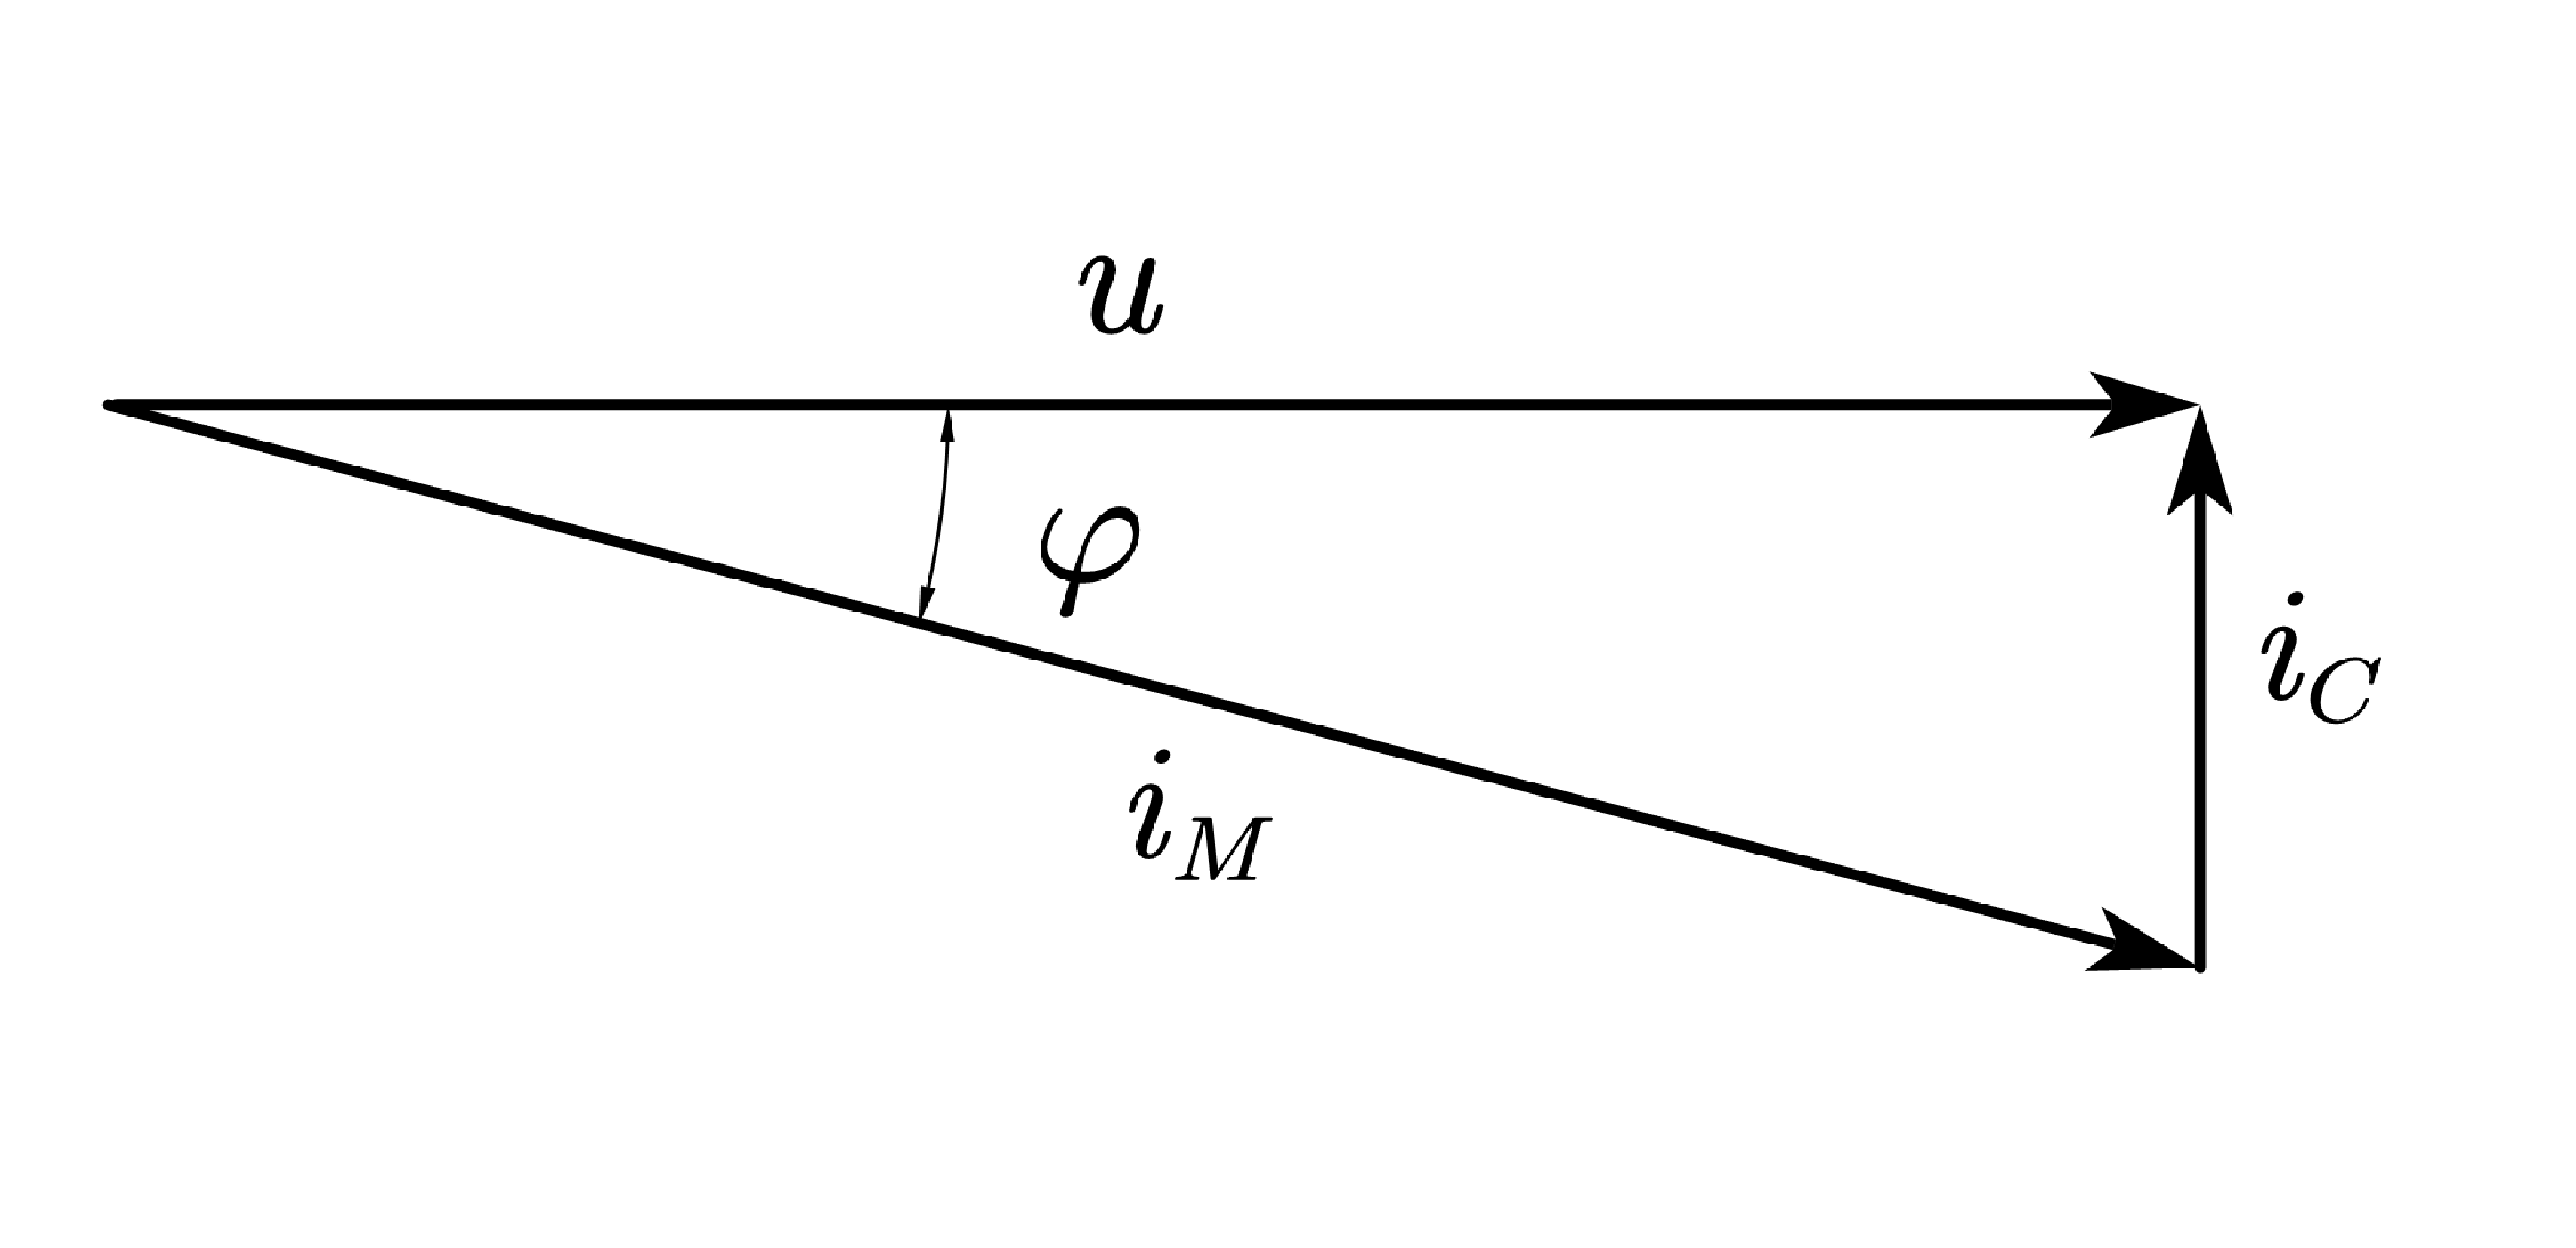
\includegraphics[width=0.7\linewidth]{8-15}
		\caption*{8-15}
		\label{fig:8-15}
	\end{figure}
	
	$$
	i_C=u\omega C=i_M\sin \varphi 
	$$
	
	$$
	C=\frac{i_M\sin \varphi}{u\omega}=2.76\,\mathrm{\mu F}
	$$
	
	\subsection*{8-16}
	
	Use defination
	
	$$
	\cos\varphi=\dfrac{P_\mathrm{in}}{\sqrt{3}ui}=0.69
	$$
	
	so
	
	$$
	P_\mathrm{var}=P_\mathrm{in}\tan\varphi=5.76\,\mathrm{kvar}
	$$
	
	\subsection*{8-18}
	
	% TODO: \usepackage{graphicx} required
	\begin{figure}
		\centering
		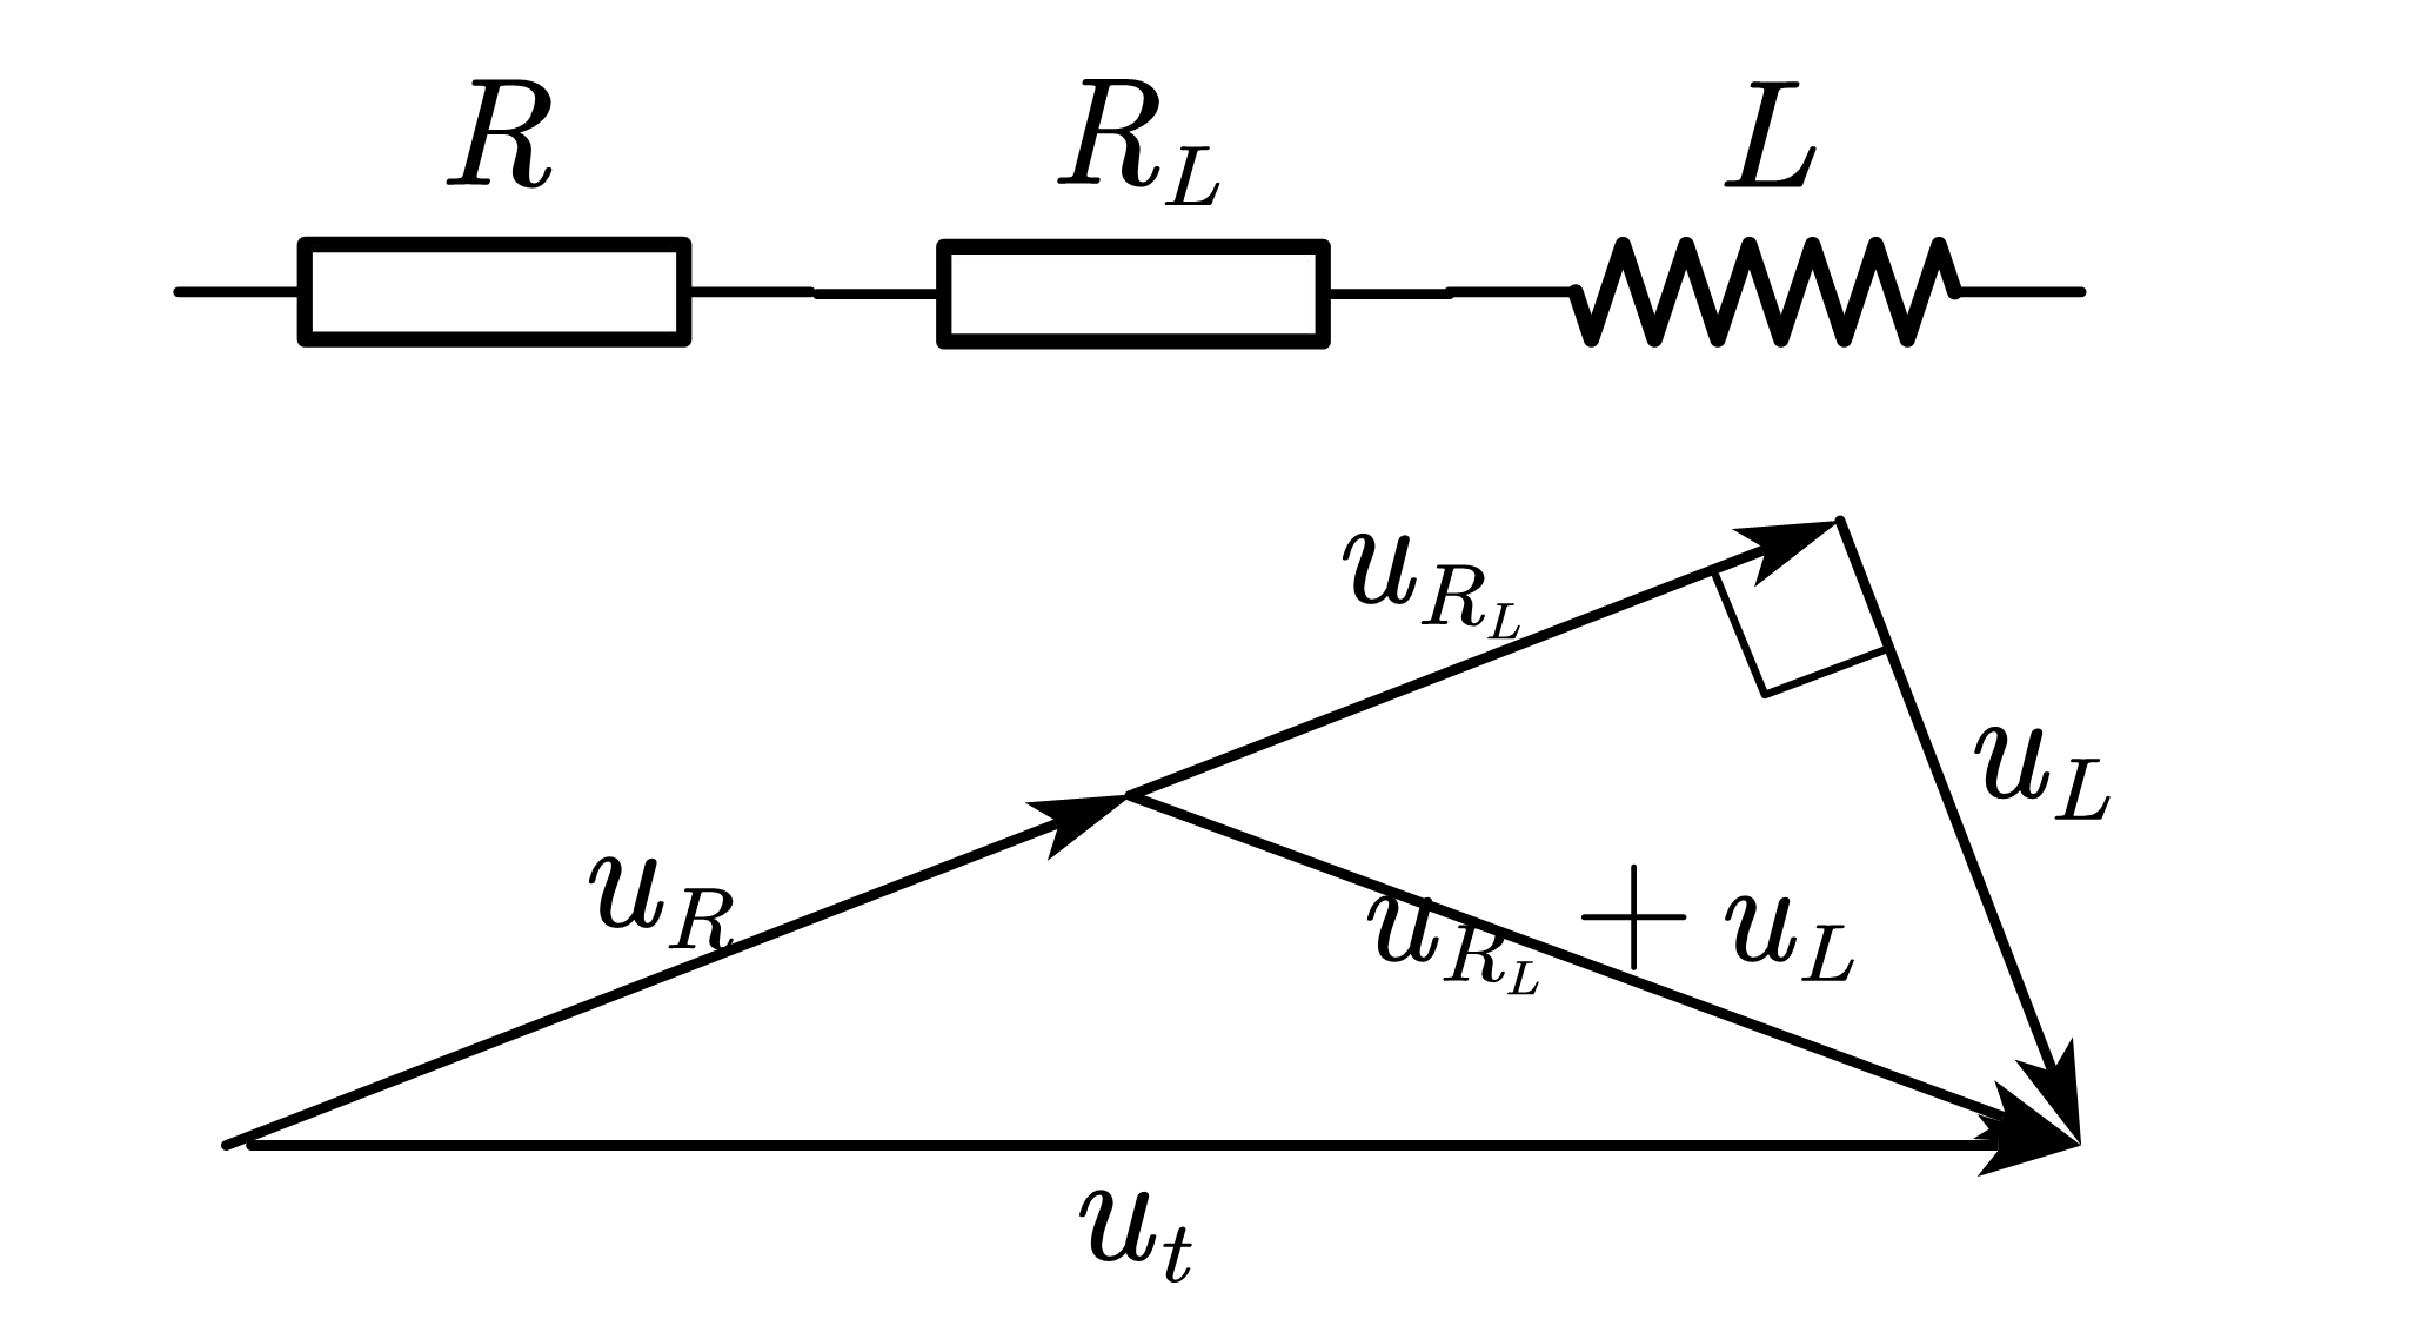
\includegraphics[width=0.7\linewidth]{8-18}
		\caption*{8-18}
		\label{fig:8-18}
	\end{figure}
	
	$$
	\left( iR_L \right) ^2+\left( \omega Li \right) ^2=\left( iR \right) ^2
	$$
	
	$$
	\left( iR_L+iR \right) ^2+\left( \omega Li \right) ^2=u_{t}^{2}
	$$
	
	So
	
	$$
	R_L=20\,\Omega
	$$
	
	$$
	L=34.6\,\mathrm{mH}
	$$
	
\end{document}

